\chapter{Discussion}
\label{discussion}

We devote this chapter to a deeper look at some of factors that may (or may not)
shed light on a few of the more perplexing and intriguing observations made
through the user studies mentioned in the previous chapter, as well as a
meta-review of what, if anything, we may conclude based on our reported data and
observations. We spend the most attention on our latest study (with the PopCAD
and SnapCAD) as it is not only the most recent, but the most significant. That
study concerns whether or not our devices can be used effectively for modeling
by novice users as well as touching on the relationships between our devices,
spatial reasoning, and embodied cognition. We start with the significance of the
gesture and speech observations made in the PopCAD and SnapCAD study, discuss
the role of age in relation to modeling performance, followed by an analysis of
the effects of shape complexity on modeling acuity, a closer look at the error
coding we performed, and finally some meta-analysis of the observed data over
the three user studies described in the last chapter.


\section{Gesture and Speech Significance}

The work of Ehrlich\cite{ehrlich2006importance}, Levine\cite{levine1999early},
and Goldin-Meadow especially\cite{goldin}\cite{goldin2005hearing}, serves as a
rough guide to our most recent study design, as they touch on the role of
gesture in determining spatial reasoning performance, and later provide strong
evidence that gesture is a valuable window into the mind, all of which supports
the notions inherent in embodied cognition - that body and mind are far more
tightly linked than we have traditionally be led to believe. As we operate under
these assumptions as reasoning to create tangible, physically involved
interfaces (as opposed to pure 2D software) it is worth taking a deeper look
into how our study results compare and contrast with this earlier work.

Ehrlich and Levine's studies focus on the gestures and speech produced during
children's explanations of how they solved a series of mental transformation
tasks. The participants were presented with the same sorts of instruments used
in our PopCAD and SnapCAD study, although our studies differ significantly in
several ways. Of course, Ehrlich and Levine had no devices, and evaluated the
speech and gestures produced in explaining the mental transformation task,
whereas we examined the strategies expressed when modeling on the PopCAD and
SnapCAD. Apart from one practice condition where wooden blocks were used (which
in their study had no effect) all of the tasks in \cite{ehrlich2006importance}
were based on 2D paper representations, and the subject had no physical contact
with any of the objects they were trying to model. In our study, subjects were
handed a 3D-printed (and thus 3D) model of the shape they were attempting to
reproduce. Additionally, in Ehrlich and Levine's studies, subjects were
instructed to (in their mind) ``move the pieces together'' or to ``observe the
movement'' of the pieces as manipulated by the experimenter. These factors, as
well as differences in age (our subject population was 5-13 years older than
those in \cite{levine1999early} and \cite{ehrlich2006importance}) likely
contribute to (at least of some of) the differences observed in our study. We
spend the next two subsections dissecting the similarities and contrasts in our
results compared to the finding reported by Ehrlich, Goldin-Meadow, and Levine.


\subsection{Contrasts}

Given the differences Ehrlich's study and own our own, it is no surprise that
our findings should differ. While the gesture and speech analyses
occurred while subjects were explaining a modeling strategy, the type of
modeling activity they had been asked to perform was substantively dissimilar.
As noted above, subjects in our study were handed physical, 3D models of the
target shape they were tasked with modeling, and could hold on to that object
(and rotate it, look at it from different angles, hold it in front of the device
or the computer screen, etc.) during their modeling process.
Afterward, when asked about their strategy, they still had that object, and
often gestured to it (or with it) and (of course) talked about it. No such
``hands-on'' activity was involved in the studies we reference above, nor (as we
note later in the chapter) could we find substantive work involving such
manipulative activities to examine spatial reasoning ability.

We contend that the ``embodied'' nature of the tasks in our study help explain
some of the differences in gesture and speech patterns and correlations that we
observed. In fact, it is likely that given Goldin-Meadow's body of work and
studies involving cognition and gesture, she would concur with us. Furthermore,
the way in which the examiner in the above studies introduces the tasks to the
subjects involves several direct references to movement (e.g. ``In your mind,
move the pieces together and then move them back apart''). This is significant,
as gestures and speech relating to movement was (in their study) both the most
frequent type of strategy expressed but, as far as gesture correlations with
task performance is concerned, gestures coded as relating to movement was the
only type of response they recorded that was exclusively related to answering
the test questions correctly. To take an excerpt from
\cite{ehrlich2006importance} (pp. 1265):
\begin{quote}
``Gesturing about moving the pieces was
correlated with the number of problems answered correctly ($r = .461,$ $p <
.001$), but it was not correlated with the number of problems answered
incorrectly ($r = .202,$ $ns$). Thus, gesturing about moving the pieces together
was uniquely related to correct performance, whereas talking about moving the
pieces was not.''
\end{quote}  

To summarize our related findings, then: in our study, gestures about movement
were the second most observed expression, after those related to perceptual
features (113 to 180); speech about movement was also second to perceptual
features in frequency (186 to 107), and neither gesture nor speech was
significantly tied to performance in our modeling tasks ($r = .29,$ $p < .29$
for gesture, $r= .27,$ $p < .32$ for speech). Instead, we found the highest
correlation (and highest frequency) in speech and gestures relating to
perceptual features ($r = .61,$ $p < .025$ for gesture, $r = .58,$ $p < .025$
for speech). Ehrlich found only a negative correlation between modeling
performance and perceptual feature coding, both from speech and from gesture.

We are then left to wonder about the rather drastic differences in our findings.
What might account for both the frequency and correlation differences in
movement versus perceptual feature strategies? Although of course we cannot know
for certain, we hinted at some of the possibilities above: the ``embodied''
nature of our tasks, having the subjects hold onto an object representative of
the solution they were striving for, the participants being' ``primed'' for
certain kinds of responses in the earlier studies, and the differences in age
all may account for some of the differences. The kind of mental processes
involved in a mental transformation task are not all that different
(necessarily) from those involved in modeling an object with the PopCAD (for
example) - a robust mental image of the shape in question is likely a boon in
either case. However, a model can be built step-by-step, and the results
observed and reflected upon. When picking a correct shape in a mental
transformation task, one may mentally operate upon features of the shape in a
step-by-step manner, but there is no opportunity to reflect upon various
strategies, a holistic decision has to be made. In a step-by-step modeling
process, it seems common (from the data and from our own experiences and
intuitions) for a modeling ``step'' to focus on a perceptual feature of the
shape being modeled (e.g. the next segment in a path or the top point in a
pyramid-shaped hull), and to do so in a very conscious way. Additionally,
subjects in our study were allowed to continue holding the model while they gave
their strategy, providing a ready ``facsimile'' on which to project their
modeling intentions. These factors may have ``paved the way'' for a high number
of speech and gesture about perceptual features of the models, as the step-wise
nature of the task and the physical surroundings lead themselves toward thinking
in terms of the characteristics of the shapes. Although we observed a high
number of expressions coded as movement, there is nothing inherently
``movement-oriented'' in 3D modeling (ones body moves in using our devices, of
course, but models can be created in other ways, e.g. strictly from text
coordinates). In contrast, a mental transformation task is, explicitly asking
the user to ``move'' the object, mentally, into the correct formation. Thus it
is unsurprising that the examiners in Ehrlich's study repeatedly used the word
``move'' and appealed to references about movement (as noted above). It is
equally unsurprising then, that by using this sort of language and then looking
at ``movement'' as a gestural and spoken strategy, many instances were found, as
the task and the instructions surrounding the task are both ``movement
oriented'' in a way that the modeling tasks in our study were not. 

One of the other major findings in \cite{ehrlich2006importance} and
\cite{levine1999early} is that significant performance differences exist between
genders on these tasks, and are evident at younger ages than previously thought.
Existing research at the time claimed that gendered differences in spatial
reasoning developed around puberty, but that several studies had challenged this
assumption. In either case, gender differences should have shown up in our study
based on the age range of our subjects (11-18). Boys did outperform girls in
session one of the modeling task,  though it was not by a terribly significant
portion (4\%), they did model faster than the girls in each round of the
modeling exercise (by about 7 minutes total in the first session, five minutes
overall in the second session), and they produced more speech instances than the
girls did overall (275 to 260), although since there were more boys in the
study, this advantage is negligible at best. Interestingly, our findings had
girls performing better in many areas; they outperformed boys in the second
modeling session by 9\%, and across both sessions by almost 3\%. Despite a
disadvantage in numbers, girls produced more gestures (225 to 188) including
those most closely linked to modeling success, perceptual features (96 to 84).
Girls also produced more speech elements about perceptual features (97 to 89).
The results from our mental transformation task have boys and girls performing
about equally, with girls edging out the boys by one tenth of a percent (85.3\%
to 85.2\%, respectively).

Was our sample size too small? Most likely, although it would be interesting to
perform a larger study with an $n$ closer to what Ehrlich and Levine had to see
if working with our devices does anything to mitigate gender effects.
Did we have an exceptionally bright group of girls? Probably, though no
independent tests were done for intelligence or other factors that would have
indicated an advantage - remember, the girls who enrolled in the study averaged
almost a full year younger than the boys (13 years, 7 months for girls and 14
years 6 months for boys), so age and experience advantages are unlikely (none of
the girls reported any previous 3D modeling experience). Although the nature of
the modeling exercises in our study were more piecemeal, possibly allowing girls
more of a chance to reflect and correct their mistakes than in the mental
transformation tasks,\footnote{There is some evidence, relayed in
\cite{ehrlich2006importance}, that girls tend to utilize a step-by-step strategy
in mental rotation problems, whereas boys tend to deal with the whole shape at
once.} we saw no significant difference in the MTT tasks we administered (in
fact girls did slightly better).

One possibility is that modeling with the sorts of devices we created are
somehow more beneficial to girls than to boys; that the spatial reasoning
advantages that boys have are either negated, or that the types of modeling
exercises we did significantly altered boys' normal spatial reasoning
strategies, which has been known to have a detrimental effect on
performance\cite{beilock2002paying}\cite{lutz2001procedural}. Plenty of other
possibilities exist (e.g., the girls simply tried harder) and there is no clear
way of determining the source(s) for our results, so we hesitate to make any
claims. However, we find it encouraging that girls were able to perform (even
out perform) when compared to the boys in our study.

\subsection{Commonalities}

Despite the differences mentioned in the previous section, some of our
observations did agree (or at least failed to disagree) with the previous
studies. In Ehrlich's study as well as ours, the study population improved
overall. In each case, girls improved by a markedly greater percentage, whereas
boys improved less so, and in some cases performance actually decreased (in our
second session overall and in the post-test for Ehrlich's ``imagine movement''
condition). Movement and perceptual feature strategies were the most common in
both studies, with perceptual whole instances far behind. Generally speaking,
gesture expressions deemed most ``task-appropriate'' (per our discussion in the
previous section) served as the highest observed correlation to modeling
success; perceptual feature gesturing in our study, movement gesturing in
Ehrlich's study. This is, we believe, the main ``gist'' of both these
experiments as far as gesture analysis goes - that gesture of a strategy
appropriate to the task at hand is correlated with success on that task, more so
than speech alone. This holds with the core of Goldin-Meadow's findings, that
gesture is a window into the cognitive process and that by analyzing gesture we
can gain insight into the mind of the learner.


% Girls improved, boys did not
% 
% Mis matchers?


\section{Age}

One of the more profound and noticeable results from the PopCAD and SnapCAD
study was the difference in modeling success between the devices in the first
round, and how much that difference was erased on the second round. In the first
session, users modeling with the PopCAD correctly modeled 75\% of the given
shapes, the highest percentage of any device in any round. Conversely, those
starting on the SnapCAD modeled only 34\% of their shapes properly. Given just
this data, we might be tempted to conclude that the PopCAD is a much easier
introductory device - or that the SnapCAD is insufferably difficult. However,
when we factor in the second round data, in which each subject modeled on the
device they did not use the first time around, a different picture emerges:
PopCAD modelers in the second round modeled 65\% of the shapes correctly while
SnapCAD modelers achieved a 56\% success rate. If we track each group (let us
call the first round PopCAD modelers group A, and the first round SnapCAD
modelers group B), we would be sorely tempted to declare that the groups
themselves are unevenly talented: Group A scored 75\% on PopCAD and 56\% on
SnapCAD, while group B scored 65\% on PopCAD and 34\% on SnapCAD. 

Since we did not perform an intelligence test or any sort of generalizable
aptitude test, we are left to guess using other means. Given the massive
development (both cognitively and physically) that occurs between the age
extremes in our subject population (11 to 18), it would be tempting (and even
logical) to assume that the older subjects would perform much better on the
modeling tasks than their younger counterparts. As it turns out, the average age
of group A was higher than that of group B - but only by three months (group A
average age was 14, group B was 13.75). We found a very modest correlation ($r =
.39, p < .15$) between age and the number of correctly modeled shapes,
suggesting that while not to be overlooked, it may play less of a role then we
would have suspected. It is also possible that the statistics are slightly
misleading here - the subject population was weighted toward the younger end of
the spectrum: the average age was 13.8, while median age was 13.5, and the mode
was 12 years old. Meaning the few older participants would have had to perform
impossibly brilliantly (i.e., higher than the highest possible score) for a
strong age to performance correlation to show up. In keeping with these
findings, we also found no real correlation between age and overall performance
on the mental transformation tasks ($r = .23, p < .45$). This data of course
does not discount that age plays a factor, nor that group A may have been more
talented than group B in the PopCAD/SnapCAD; simply that within rough
parameters, age matters, just not as much as one might think. Take for example
our oldest participant, an 18 year-old boy. He correctly performed 11 of the 24
modeling tasks, while the four 12 year-old participants scored 14, 11, 12, and
11. Our youngest participant, and 11 year old, reproduced seven shapes
correctly, while a 13 year old did five correctly, and a 14 year old got six
right.


\section{Shape Complexity}

In order to attempt to judge each shape's complexity, we sought out a
previously-defined set of criteria by which to judge ``complexity''. As it turns
out, there is a long and thorough discussion of complexity in relation to
\emph{two-dimensional} shapes, starting seemingly with Fred Attneave and Malcolm
Arnoult\cite{attneave1956quantitative}\cite{attneave1957physical} in the mid
1950's, who define methods of generating random two-dimensional shapes and
examine their physical characteristics in relation to their judged complexity.
As it turns out (in \cite{attneave1957physical} as well as others' follow-up
work) the ``Number of Turns'' in the shape was responsible for significant
amount (nearly 80\% in Attneave's study) of the preceived complexity of a shape.
``Number of Turns'' is defined as ``the number of maxima (regardless of sign)
in one cycle of the function relating curvature to distance along the contour.
This function is a series of spikes for any angular shape, and a step-function
for any curved shape\ldots'' (see p. 226 of the aforementioned article).
Symmetry, angular variability, and squared perimeter over area also had some
effect.

However, as it seems unclear to us how one might adapt a ``Number of Turns''
rating to a true \emph{three} dimensional model. Many studies claim to have
studied complexity in relation to 3D mental transformation tasks, (starting with
Shepard and Metzler\cite{shepard1971mental}), but they (as well as the many
other studies we
found\cite{metzler1974transformational}\cite{shepard1988mental}\cite{vandenberg1978mental}
used perspective line drawings, \emph{not} actual physical models. This had an
advantage for the types of mental rotation tasks they were performing
(recognition of matching pairs), but seemed insufficient for the tasks in our
study.

This led us to develop (as best we way) a rubric to determine the complexity of
the shapes we presented in the study, as a way of teasing out any correlation
between complexity and performance. In lieu of attempting an exact number of
turns estimate, we included three criteria: (a) the minimum number of lights
necessary to guarantee the correct shape,\footnote{In minimal spanning tree
models where a placement of lights results in several possible correct
formations, only one of which is the desired shape, we add points necessary to
``force'' the correct representation.} (b) the number of faces (for convex hull
models only), the number of line segments (for path models only), or the number
of distinct branches (for tree models only), and (c) a symmetry score based on
number of lines of symmetry, from 3 (indicating asymmetry) to 0 (indicating
three or more lines of symmetry). The scaling for symmetry comes from the belief
that indicators (a) and (b) above are more closely aligned with Attneave's
``number of turns'' metric (being highly correlated to perceived difficulty),
while symmetry was much less correlated to complexity (although symmetry did
still play a part), so we made the scale as low as possible so that it would
weigh less on the overall complexity score of a model. So, for example, a
regular octahedron would have six points, eight faces, and a zero symmetry score
for an overall difficulty score of 14. The complexity score of each shape is
shown in \ref{modelComplexity} next to the number of times it was modeled
correctly. The shapes in each session were of course different, but are labeled
the same in this table, indicating the order in which they were presented.

\begin{table}[!ht] 
\small
    \caption[Complexity of Models and Modeling Performance]{Complexity of Models
    and Modeling Performance (CH = Convex Hull, P = Path, T = Minimal Spanning
    Tree)}
    \begin{center}
    \begin{tabular}{| c | c | c | c | c | c | c | c | c | c | c | c | c | }
    \hline $ $ & CH1 & CH2 & CH3 & CH4 & P1 & P2 & P3 & P4 & T1 & T2 & T3 & T4 \\
   	\hline
   	$Session$ $1$ & & & & & & & & & & & &  \\ \hline
   	$Complexity$ $Score$ & 14 & 19 & 19 & 19 & 7 & 18 & 20 & 24 & 9 & 13 & 17 &
   	17 \\ \hline 
   	$Performance$ of 19 & 8 & 13 & 8 & 11 & 17 & 14 & 8 & 9 & 12 & 8 & 8 & 11 \\
   	\hline 
   	$Session$ $2$ & & & & & & & & & & & & \\ \hline
   	$Complexity$ $Score$ & 12 & 20 & 15 & 13 & 14 & 14 & 18 & 17 & 21 & 17 & 16
   	& 25 \\ \hline 
   	$Performance$ of 16 & 7 & 9 & 11 & 11 & 11 & 13 & 8 & 12 & 7 & 11 & 7 & 9 \\
   	\hline
   	
	\end{tabular}
   \\ \rule{0mm}{5mm}
\end{center}
\label{modelComplexity}
\end{table}


One might expect to see a strong negative correlation between a given model's
complexity score and the number of subjects who were able to model it correctly,
however the observed correlation was only moderate: $r = -0.41, p < .05$ over
both sessions, indicating that while shape complexity (at least as we have
calculated it) is significantly correlated, it plays only a moderate role in
determining modeling performance in our study.


\section{Freehand Modeling}

At the end of both sessions, the subjects were given the opportunity to model a
shape of their own design, using any of the modes presented during the modeling
exercises. Each participant modeled after the first round, and then were given
the opportunity to create a different shape after the second round that they
wanted printed out instead (most subjects stuck with their original model). The
prints from the 16 participants who finished the study are shown in Figure
\ref{UserShapesAll}.

\begin{figure}[!ht]
\begin{center}
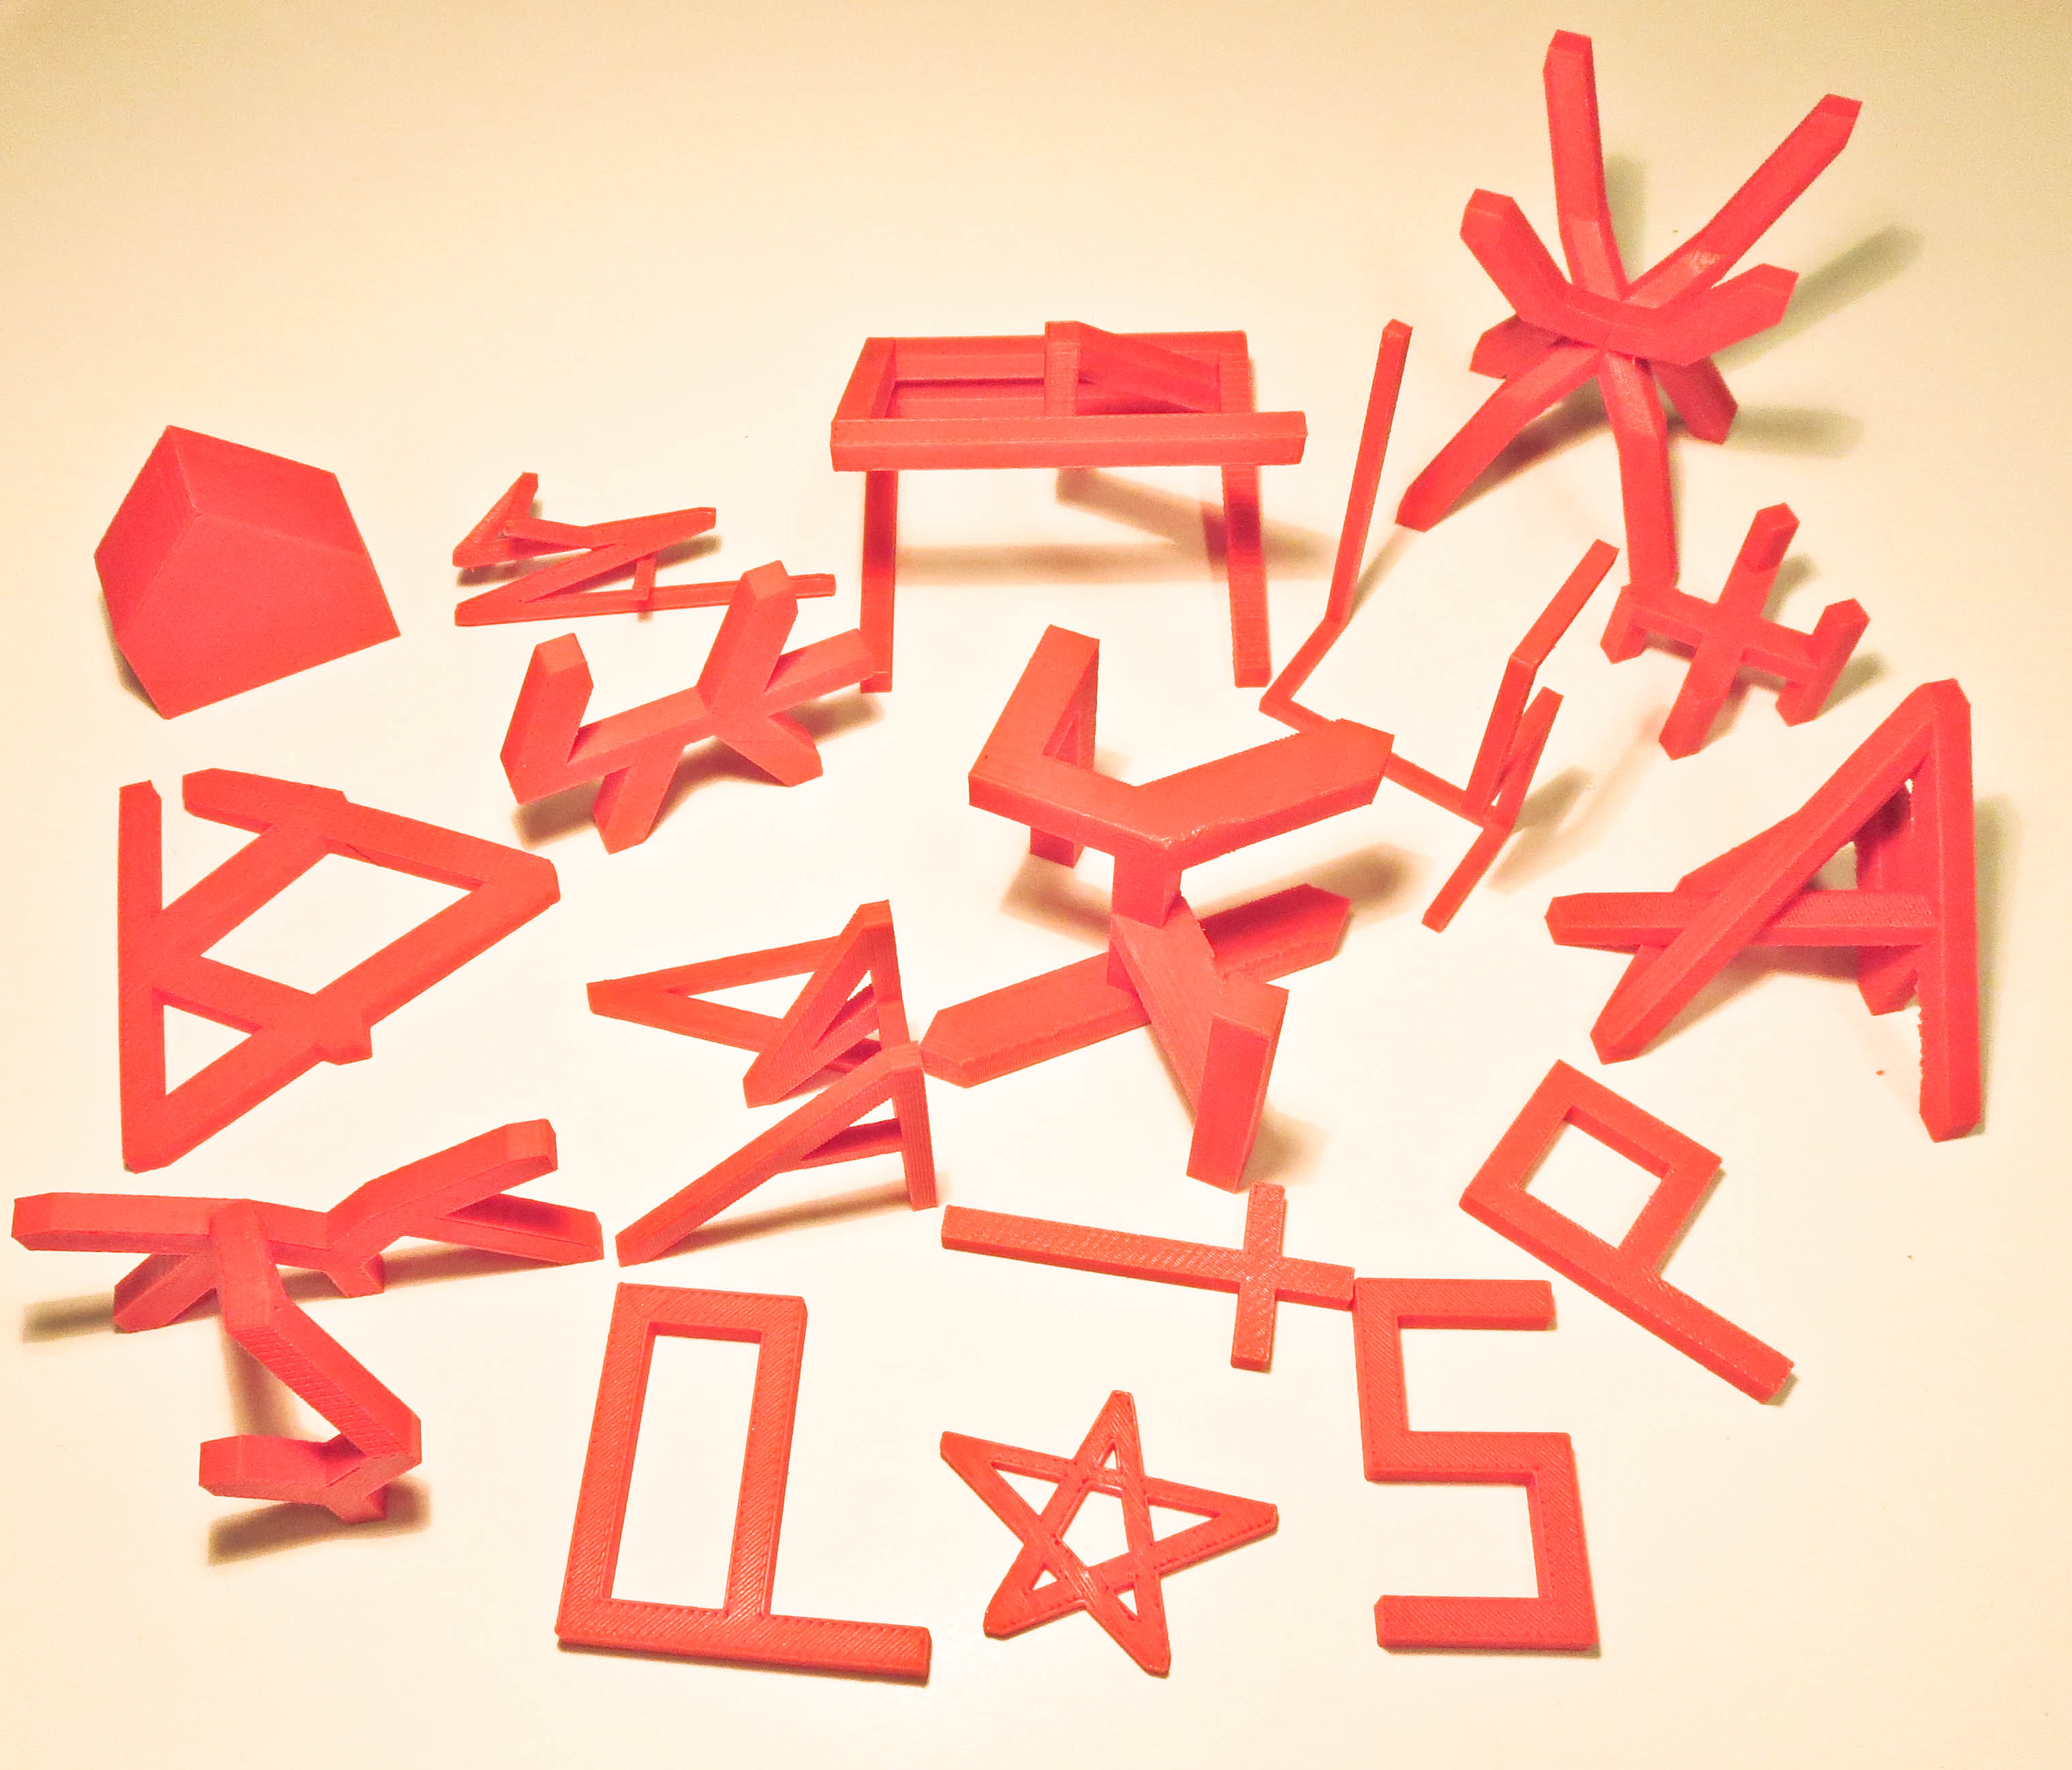
\includegraphics[width=.55\linewidth]{images/userShapesAll} 
\end{center}
\caption{A collection of the child-designed objects from the PopCAD/SnapCAD
study.}
\label{UserShapesAll}
\end{figure}

Objects were created using all three modes, though only one participant chose
the convex hull mode for their object; nine subjects used the path mode, while
six used the minimal spanning tree mode. It should be noted that almost every
participant explored all three modes on their own before settling on one they
liked the best. Choices were sometimes based on strategy (e.g. only one mode was
capable one making the shape they envisioned) while many users simply explored
different modes and patterns until something struck their fancy.
As evident in the picture, some users went with letters (usually the initial of
their first name), others attempted to create a symbol they knew (e.g. one
participant attempted the ``Tri-Force'' symbol from the Zelda video game
franchise), and others (as hinted at in Figure \ref{UserShapesAll}) simply
turned points on and off until they achieved an aesthetically pleasing object.

Of the 24 user-created models (19 from the first session, 5 more from the second
session) we received an even number generated from each device (12 apiece). We
were curious to see if, on the SnapCAD models, users took advantage of the
greater expressive power offers by the larger input space (a $7^3$ grid compared
to a $3^3$ grid). Of the 12 SnapCAD models, 9 of them would have been impossible
to model using the PopCAD (without substantial use of the editing mode, at
least).\footnote{Two notes here: (1) We counted the shape as impossible if any
vertices would have to change planes to create the shape; (2) Any shape modeled
on PopCAD can, of necessity, be recreated on SnapCAD.} Of the five users who
chose to model a new shape after the second round, four of them had used PopCAD
in the first round and SnapCAD in the second round.
Three of these four users modeled shapes they would not have been able to using
PopCAD. However, based on the difficulty rubric laid out in the previous
section, the average complexity of shapes modeled on the PopCAD was actually
higher than that of SnapCAD (22.83 to 18.50). Interestingly though, the shapes
with the three highest scores (all from PopCAD) were from users who chose to
model different shapes after the second round in order to use the SnapCAD - but
to create a ``simpler'' shape (i.e., a shape with a lower complexity score).
Granted, there are some mitigating factors at work here - on the PopCAD
interface, it is fairly straightforward to turn on all 27 points - it is a
simple touch of the finger, the lights are already placed on the towers. On
SnapCAD, more effort is required to take a tower, place it into a socket, take
an LED board, and then snap it onto a location on the tower. In fact, several of
the high scores we just referred to were generated by users simply turning on
all the lights with path or tree mode active. If we compare the set of PopCAD
models without those models dropped in favor of SnapCAD models after the second
session, the shape complexity average drops to 16.75 - a few points less than
the SnapCAD average.

Interestingly, most of the ``intentional'' models - those models created from a
firm mental model or notion of what the final shape should be - a preferred
strategy was to use the path mode and a singular vertical plane (e.g. the first
row of three towers on the PopCAD) to treat the device essentially as a
2-dimensional drawing tool. We can see (in the figure above) shapes like the
star, or the letter ``s'' - while they print in 3D of course, the modeling
necessary to create these shapes happens in 2D. Also of note is that the users
overwhelmingly chose a vertical (as opposed to horizontal) plane in which to
work. When we imagine ourselves drawing or writing, it is almost along a flat
horizontal surface (except perhaps when writing on a whiteboard or painting on
an easel), so why the preference for verticality? While we cannot know for
certain, it is true that some amount of verticality is implied in the device -
the towers themselves rise in vertical columns above the ``floor'' of the
device. Additionally, the average time writing manually as opposed to typing on
a computer has significantly decreased in recent years, so perhaps the vertical
screen of a computer somehow relates. In any event, using the device as more of
a 2D drawing instrument is a somewhat unexpected, but nonetheless welcome
observation.

The freehand modeling session (or sessions) were quite clearly the most
enjoyable for the users themselves. None of the participants refused to do the
freehand modeling session, or quit in the middle of it. In fact, many subjects
went over the allotted 10 minute modeling window exploring, testing ideas,
rearranging point configurations, and generally being absorbed by the
experience, which we found encouraging (and of course we allowed subjects to
play as long as we could). This suggests some viability for a device like this
in a classroom (especially one with a desktop 3D printer), where students could
simply play with the interface, observe the interactions between 2D and 3D
representations in a fluid manner, and print their own creations with the click
of a button.


\section{Error Analysis}

For each modeling task, one (and only one) of seven error codes was recorded,
based on the outcome of the task. A more complete detail of the error codes can be
found in table \ref{modelingError}; this section focuses instead on what significance
(if any) these error codes have on our observations\footnote{Again, this data
is from the PopCAD/SnapCAD study only.}. To briefly recount the codes and their
associations, then: C = correct, EP = error in proportion (general shape is
correct, but model is too tall, too wide, etc.), E1 = error in recognition
(subject had the correct shape but did not recognize it), E2 = error in belief
(thought the shape was correct when it was not), E3 = error in implementation
(knew shape was incorrect, but knew why), E4 = error in strategy (subject knew
shape was incorrect, but could not explain why), I = incomplete (includes
giving up, asking to move on, running out of time).

\begin{table}[!ht] 
\small
    \caption[Modeling Error Code Breakdown]{Error Code Breakdown. C = Correct,
    EP = Error in Proportion, E1 = Error in Recognition, E2 = Error in Belief,
    E3 = Error in Implementation, E4 = Error in Strategy, I = Incomplete.}
    \begin{center}
    \begin{tabular}{| c | c | c | c | c | c | c | c |}
    \hline $ $ & $Total$ & $Session$ $1$ & $Session$ $2$ & $PopCAD$ & $SnapCAD$
    & $Girls$ & $Boys$\\ \hline 
    $C$  & 243 & 127 & 116 & 152& 91 & 100 & 143 \\ \hline
	$EP$ & 44  & 19  & 25  & 16 & 28 & 20  & 24 \\ \hline
	$E1$ & 1   & 1   & 0   & 0  & 1  & 1   & 0 \\ \hline
	$E2$ & 50  & 28	 & 22  & 20 & 30 & 13  & 37 \\ \hline
	$E3$ & 2   & 2   & 0   & 0  & 2  &	0  & 2 \\ \hline
	$E4$ & 17  & 9   & 8   & 7  & 10  & 6   & 11 \\ \hline
	$I$  & 63  & 42  & 21  & 21 & 42 & 28  & 35 \\ \hline
	\end{tabular}
   \\ \rule{0mm}{5mm}
\end{center}
\label{modelErrors}
\end{table}

As we can see from Table \ref{modelErrors}, several types of errors barely
occurred (errors in recognition and errors in implementation), while others were
more common (proportional errors, belief errors, and incomplete tasks). As a
designer, it is comforting that errors in which the user had the correct answer
but was unable to recognize it and errors in which the subject knew the correct
strategy to model the shape but could not implement it (E1 and E3, respectively)
were minimal, as these errors seem to point more towards a failure of the
interface (the software representation being unclear, or the modeling mechanisms
being hard to use) as opposed to genuine difficulty in modeling the shape.
Interestingly, although not significant statistically because of their sparsity,
E3 codes actually had a mild positive correlation to modeling success ($r=.31,$
 $ns$), possibly indicating that correct expression of strategy in cases of
error are positive pointers towards modeling success in other cases.

Incomplete codes tell us little about the beliefs or modeling strategy of the
user beyond an inability (or unwillingness) to model the shape in the given
time. Unsurprisingly, ``I'' codes present a very high negative correlation with
modeling success, as no other strategy code could be applied ($r=-.825,$ $p <
.001$). As we might have guessed, a bad strategy is better than none at all:
code E4, where users knew their model was incorrect, yet expressed a strategy
(albeit one that would not have yielded the correct solution) was still
negatively correlated with overall modeling success, but less so than ``I''
coded results ($r=-.610,$ $p <.013$). E4 codes also carried a weaker negative
correlation than E2 codes, where the user mistakenly believed they had modeled
the shape properly (unlike in E4 codes, where the user was aware the shape was
wrong). E2 codes were the second most negatively correlated error to modeling
success ($r=-.764,$ $p < .001$).

While developing the coding system described above, it seemed important to
separate instances where the modeler had modeled the shape properly
\emph{except} for an error in proportionality, instead of simply lumping them
into the E2 code. This kind of error was fairly common, occurring 44 times in
our study, and seemed to represent its own unique category, although we were
unable to find related literature to support this. However, of the categories
with more than a few instances, errors in proportion were the least negatively
correlated to success on the modeling tasks ($r=-.235,$ $p < .390$), somewhat
justifying our belief that errors in proportion only were of a different breed
of mistake. This likely stems from the fact that unless a user asked directly if
proportion in the models mattered, they were not told that it did.
This means that several users who repeatedly made EP errors may have been able
to fix their models had they known that proportionality was a factor.
Occasionally, during the explanation of their modeling strategy, users who had
an EP error would realise or express that they could have modeled the shape more
accurately (and sometimes even fix it on the spot), in which cases modeling
times and error codes were adjusted accordingly. Although we cannot present
direct evidence why errors in proportion are less harmful than the other sorts
of errors we recorded, it does seem somehow intuitive to us that this should be
so; a triangular prism that is wider than the model presented is still a
triangular prism - it is not a cube, or tetrahedron - there is not an error in
``kind'' - merely one of scale. A mismatch in proportion only seems to imply a
greater degree of understanding and modeling ability than simply misrepresenting
the intended shape completely, and the data we have collected seem to bear
this out. Although none of these findings are particularly surprising on their own,
it is worth noting that the kinds of errors modelers make are very often
indicative of their overall performance.

\section{Cross-Study Comparisons}

The three studies mentioned in the last chapter are quite different in most
respects. The first two UCube studies have much more in common with each other
(obviously) than with the PopCAD/SnapCAD study, yet it is worth looking at the
results from all three to investigate what, if any, larger patterns emerge.


\begin{table}[!ht] 
\small
    \caption[Cross Study Comparisons]{Cross Study Comparisons.}
    \begin{center}
    \begin{tabular}{| c | c | c | c | c | c | c |}
    \hline $ $ & $Subjects$ & $Ages$ & $Modeling$ $Modes$ & \#
    $Models$ & $Correct$ & \% \\ \hline 
    $UCube$ $Pilot$  & 14 (6 groups) & 12-14 & Convex Hull & 5 & 24/30 & 80\% \\
    \hline 
    $UCube$ $Follow-Up$  & 10 (indiv.) & 11-13 & Convex Hull & 5 & 41/50 & 82\% \\ \hline 
    $PopCAD/SnapCAD$  & 20 (indiv.) & 11-18 & C.Hull, Path, Tree & 24 & 243/420
    & 57.9\%
    \\
    \hline

	\end{tabular}
   \\ \rule{0mm}{5mm}
\end{center}
\label{crossStudy}
\end{table}


When we compare raw modeling performance across studies, we see the first study
resulted in 80\% (24 of 30) correct models, the second UCube study resulted in
82\% (41 of 50), while the third study resulted in only 243/420, or about 58\%.
The last study is of course the outlier, but the above table includes models
from the other modes (Path and Tree), that the other two studies did not
examine. If we compare only across convex hull modeling tasks, the
PopCAD/SnapCAD study yields eight models across both modes, with 78/140 convex
hull tasks modeled correctly, or 56\%. While much lower than the earlier studies,
this number still ignores the differences between devices. Convex hull models
on the PopCAD were correct 30/40 times in the first round and 17/32 times in the
second round, for a total of 47/72 for a little over 62\%. SnapCAD produced
10/36 correct models in the first session and 21/32 in the second round, or
31/68 or abut 46\%. Interestingly, neither of these numbers is particularly
close to the convex hull success we observed in the earlier UCube studies.

What might explain this discrepancy? Are the PopCAD and SnapCAD devices really
that much harder to use, or could there be another explanation? One possibility
worth looking at is the shape complexity metric we developed in the previous
section, as we noticed a moderate negative correlation between shape complexity
and modeling score, suggesting that if we the models were much easier in the
easier studies, some of the difference in score might be attributed to that
relationship.

As a brief reminder, then: the complexity score for a convex hull is the sum of
the number of points and faces plus a symmetry score (three points for
asymmetry, two points for one-axis symmetry, one point for two-axis symmetry,
and no points for more than two-axis symmetry). To report the complexity scores
(breakdown of points, faces, and symmetry score is given for the two studies not
previously disclosed):
\begin{quote}
	$UCube Pilot:$ 2 (2+0+0), 2 (2+0+0), 14 (8+6+0), 12 (6+5+1), 11 (4+4+3) \\
	41 / 5 = 8.2 complexity average \\
	\\
	$UCube Follow-Up:$ 14 (8+6+0), 8 (4+4+0), 14 (6+8+0), 18 (9+9+0), 18 (9+6+3) \\
	72 / 5 = 14.4 complexity average \\
	\\
	$Pop/Snap:$ 14, 19, 19, 19, 12, 20, 15, 13 \\
	131 / 8 = 16.375 complexity average \\
	
\end{quote}

While the PopCAD/SnapCAD study did in fact have the greatest average complexity
score, it beat out the highest performing study (the UCube follow-up) by less
than two points. Given the 20\% plus drop a two-point difference does not seem
to be able to explain it all, especially given that the highest performing study
did not have the lowest complexity score (the first pilot did). However, one
mitigating factor may be that four of the shapes in the PopCAD/SnapCAD study
were harder than the hardest shapes encountered in the UCube follow-up study. It
could be that performance is relatively linear up until a certain complexity
point, after which it drops dramatically. We also used more ``standard''
polyhedrons in the UCube follow up, many of which have a ``deceptive''
complexity score; a cube, for example, may be the easily recognizable and most
easily modeled shape (it was in the UCube follow-up study), but it has a
complexity score of 14, more than the ``right-angle'' off centered pyramid we
used in the PopCAD/SnapCAD study. Moreover, we did not use a cube in the
PopCAD/SnapCAD study, while it was used in both of the UCube studies. Another
possibility is that, given the smaller sample size and fewer models, we simply
did not take a large enough sample in the first two studies. The pilot had six
groups over five shapes (30 tasks), the follow-up UCube study had five tasks
with ten individuals (50), while the PopCAD/SnapCAD study had four tasks over 19
individuals in the first session and four tasks over 16 individuals in the
second round for a total of 140 tasks - almost three times the size of the UCube
follow-up. It is possible that if we had performed a larger number of tasks in
the earlier studies that the performance numbers would start to move closer to
what we observed in the PopCAD/SnapCAD study.

Finally, one last factor to take into account here are the subject demographics.
Only two participants in the PopCAD/SnapCAD study had indicated previous
experience with 3D modeling in any capacity, and the study site was a drop-in
program serving primarily disadvantaged youth in a predominantly low
socioeconomic neighborhood (indeed, one of the neighborhood schools was
scheduled to close permanently while we conducted our study). In contrast, the
two earlier studies with the UCube were performed at a fairly affluent,
predominantly Caucasian middle school, with students from a multimedia class,
most of whom had been exposed to 3D modeling software (like Google
SketchUp\cite{SketchUp}) as part of their classroom multimedia curriculum.
Additionally, the UCube follow-up study was skewed in gender more so than the
other studies (eight boys to two girls) and since boys tended to do better on
modeling tasks, especially upon their first interactions - the UCube studies
only had one session - this gender balance may have played a role in the
modeling performance we observed. Although these factors are merely speculative,
the observed performance (in the 80\% range for the middle school subjects and
less than 60\% for our drop-in program), is likely not all due to innate
modeling ability, differences in shape complexity, or the use of the UCube
device specifically.

\section{A Note On Other Uses}

Thus far we have focused on our devices as a means of engaging novices in design
for 3D printing. However, that is not the only (or potentially even the best)
use case for these instruments. From a pedagogical perspective, it is easy to
think of several areas to which devices like ours may be well-suited.
In mathematics instruction, the grid-like properties of the interfaces seem to
be a very ``natural'' way to introduce (for example) 2D and 3D coordinate
systems, simple linear graphs, the notions of slope, axes, and origin, geometric
shapes (like a cube or a trefoil knot) and relations (like perpendicularity or
symmetry), and many more. In chemistry, molecules could be visualized using the
minimal spanning tree mode; in astronomy, constellations could be modeled.
More literally, in art, base components could be made for sculpture and scale
models of bigger pieces; architecture students could print out basic shapes for
their building structures and scenes. The diversity of use cases underscores how
powerful these sorts of devices (even the simple ones) can be. In the following
chapter we discuss in more detail a few more ideas about what the future
of embodied fabrication devices might look like.
